\chapter{Measuring exponents from finite data}
\label{ch:measuring}

\newcommand{\stestLSlinMean}{0.893}
\newcommand{\stestLSlinStd}{0.124}
\newcommand{\stestLSlogMean}{1.907}
\newcommand{\stestLSlogStd}{0.080}
\newcommand{\stestLScumMean}{1.992}
\newcommand{\stestLScumStd}{0.032}
\newcommand{\stestMLEMean}{2.000}
\newcommand{\stestMLEStd}{0.023}
\newcommand{\stxminBest}{10.0}
\newcommand{\stxminTau}{2.496}
\newcommand{\stxminErr}{0.011}
\newcommand{\stxminTauOne}{1.58}
\newcommand{\stbtwWinTau}{1.123}
\newcommand{\stbtwWinErr}{0.002}
\newcommand{\stbtwWinP}{0.15}
\newcommand{\stcorrRatio}{0.2}
\newcommand{\stcorrAcfOne}{-0.007}
\newcommand{\stcorrSeed}{0.14}
\newcommand{\stsynTau}{1.608}
\newcommand{\stsynD}{2.056}
\newcommand{\stsynCost}{0.8}
\newcommand{\stmomD}{2.81}
\newcommand{\stmomTau}{1.29}
\newcommand{\stmomCost}{1197}
\newcommand{\stcollATau}{1.15}
\newcommand{\stcollAD}{2.21}
\newcommand{\stcollACost}{109}
\newcommand{\stcollBTau}{1.69}
\newcommand{\stcollBD}{3.21}
\newcommand{\stcollBCost}{3}
\newcommand{\stDloc}{2.70, 2.69, 2.88, 2.73}
\newcommand{\stDerr}{0.02, 0.04, 0.05, 0.08}


The previous chapter showed that the central claims about a critical system are statements about
exponents: the exponent $\tau$ of the size distribution, the exponent $D$ that says how the cutoff
grows with the system size. A simulation produces a finite list of numbers, and turning that list
into an exponent with an honest error bar is harder than it looks. Three difficulties appear in
every case:
\begin{enumerate}[nosep]
  \item \textbf{Statistical noise.} Large events are rare, so the tail of a distribution is always
    poorly sampled.
  \item \textbf{A finite range.} The power law holds only between a lower scale (the lattice, one
    block) and an upper cutoff (the system size, the correlation length). Outside this range the
    distribution bends, and a fit that ignores this is biased.
  \item \textbf{A finite system.} Even inside the range, the exponents measured at finite size
    differ from their asymptotic values by \emph{corrections to scaling} that disappear only slowly.
\end{enumerate}
A fourth, more technical difficulty is that consecutive events in a simulation are not independent.

This chapter develops the methods used in the rest of the thesis to deal with these problems. To
know whether a method works, it must be tried on data whose answer is known. We therefore test every
method first on \emph{synthetic data}, random numbers drawn from a distribution chosen by us, and then
apply it to the two-dimensional BTW sandpile of Chapter~\ref{ch:soc}. The methods follow
Clauset, Shalizi and Newman~\cite{Clauset2009}, Newman~\cite{Newman2005}, and the standard literature on
finite-size scaling. The chapter ends (\cref{sec:protocol}) with the procedure adopted for the
Burridge--Knopoff model.

% ======================================================================
\section{Estimating a probability density: histograms}
\label{sec:histograms}

\subsection{Counts and densities}

Suppose we have $N$ measured values $x_1,\dots,x_N$ (for example, the sizes of $N$ avalanches). To estimate
the probability density $P(x)$, divide the $x$-axis into intervals called \emph{bins}, with edges
$e_0<e_1<\dots$, and count the number $n_k$ of values that fall into bin $k$, the interval $[e_k,e_{k+1})$.
The fraction $n_k/N$ estimates the probability of falling into the bin, which is $\int_{e_k}^{e_{k+1}}P(x)\,\dd x
\approx P(x)\,w_k$, where $w_k = e_{k+1}-e_k$ is the width of the bin. Hence
\begin{equation}
  \hat P(x_k) = \frac{n_k}{N\,w_k}
  \label{eq:hist}
\end{equation}
is an estimate of the density at a point $x_k$ inside the bin. Dividing by the width is essential: without
it, wider bins would show more counts simply because they are wider.

\paragraph{The error of a bin.} Each of the $N$ values falls into bin $k$ with a small probability, independently
of the others. The number $n_k$ is then (to a very good approximation) a \emph{Poisson} random variable, whose
standard deviation is the square root of its mean. The statistical error of a bin is therefore
\begin{equation}
  \delta n_k \approx \sqrt{n_k}, \qquad \frac{\delta\hat P}{\hat P} = \frac{1}{\sqrt{n_k}}.
\end{equation}
A bin with 100 counts is known to 10\%; a bin with one count is known only to within a factor of two or so.

\subsection{Linear and logarithmic bins}

The simplest choice is bins of equal width. For a power law this is a poor choice (\cref{fig:binning}, left).
Because $P(x)$ falls by many orders of magnitude, the bins in the tail contain zero or one event. Bins with
zero events cannot even be drawn on a logarithmic axis, and those with one event pile up on a horizontal line
at $\hat P = 1/(Nw)$: the ``floor'' of the histogram. This floor has nothing to do with the true distribution.

\begin{figure}[t]
  \centering
  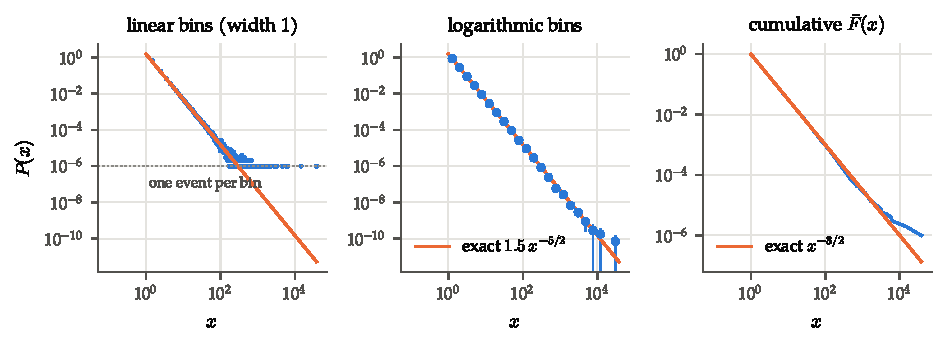
\includegraphics[width=\linewidth]{stats/binning.pdf}
  \caption{One million values drawn from the power law $P(x) = 1.5\,x^{-5/2}$, $x\ge1$, shown in three ways.
  Left: bins of width 1; the tail is dominated by bins with a single event (dotted line). Middle: logarithmic
  bins, five per decade, with Poisson error bars. Right: the complementary cumulative distribution, which needs
  no bins.}
  \label{fig:binning}
\end{figure}

The remedy is \emph{logarithmic binning}: bins whose edges are equally spaced in $\log x$,
\begin{equation}
  e_k = x_{\min}\, 10^{k/m},
\end{equation}
with $m$ bins per decade. The width of a bin is then proportional to its position, $w_k\propto e_k$, so bins in
the tail are wide and collect many events. For a power law the expected count in a bin is
$N P(x) w \propto x^{-\tau}\cdot x = x^{1-\tau}$, which falls much more slowly than $P(x)$ itself. On a log--log
plot the bins are equally spaced, and the points have comparable error bars over many decades
(\cref{fig:binning}, middle).

For \emph{integer} data such as numbers of topplings, the edges must be rounded to integers, and the width $w_k$ in
\cref{eq:hist} is the number of integers in the bin; otherwise the first few bins, which contain only one or two
integers, are distorted.

\paragraph{The magnitude histograms of Carlson and Langer.} Carlson and Langer plot the frequency of events as a
function of $\mu = \ln M$, using bins of equal width in $\mu$. Equal bins in $\ln M$ are exactly logarithmic bins in
$M$. Their density per unit $\mu$ is $\mathcal R(\mu) = M P(M)$ (\cref{eq:CL-b-tau}), so for a power law
$\mathcal R \propto M^{1-\tau} = e^{-(\tau-1)\mu}$. A straight line of slope $-b$ in their plots therefore
corresponds to
\begin{equation}
  \tau = 1 + b ,
\end{equation}
as found in Chapter~\ref{ch:intro}.

\subsection{The cumulative distribution}

The complementary cumulative distribution $\bar F(x)$ is estimated without any binning: sort the values, and for
the $r$-th smallest value set $\hat{\bar F}(x_{(r)}) = (N-r+1)/N$, the fraction of values at least as large.
For a power law $\bar F\propto x^{-(\tau-1)}$ (\cref{eq:Fbar-pl}), a straight line on a log--log plot
(\cref{fig:binning}, right). The cumulative plot is smooth and is very useful to judge by eye whether the tail
follows a power law. Its points are, however, strongly correlated with each other, since each point counts all
the values above it; this matters when a line is fitted through them.

% ======================================================================
\section{Why straight-line fits on log--log plots fail}
\label{sec:ls}

The most common way to estimate an exponent is to fit a straight line through the points of a log--log plot by
least squares and read off the slope. Least squares is the right method when the points are independent and have
Gaussian errors of the same size. None of these conditions holds here:
\begin{itemize}[nosep]
  \item the relative error of a histogram bin, $1/\sqrt{n_k}$, varies by orders of magnitude between the
    head and the tail, and the error of $\log n_k$ is not Gaussian when $n_k$ is small;
  \item empty bins must be discarded (their logarithm is $-\infty$), which removes precisely the bins that are
    below average and biases the tail upwards;
  \item the points of a cumulative plot are not independent.
\end{itemize}

To see how much this matters, we drew 1000 independent samples of $N=2000$ values each from a power law with
$\tau = 2$ and $x_{\min}=1$, and estimated $\tau$ in four ways for every sample. The results are shown in
\cref{fig:estimators}:

\begin{center}
\begin{tabular}{lcc}
\toprule
method & mean of $\hat\tau$ & spread (std) \\
\midrule
least squares, linear bins of width 1 & \stestLSlinMean & \stestLSlinStd \\
least squares, logarithmic bins & \stestLSlogMean & \stestLSlogStd \\
least squares, cumulative distribution & \stestLScumMean & \stestLScumStd \\
maximum likelihood (\cref{sec:mle}) & \stestMLEMean & \stestMLEStd \\
\bottomrule
\end{tabular}
\end{center}

\begin{figure}[t]
  \centering
  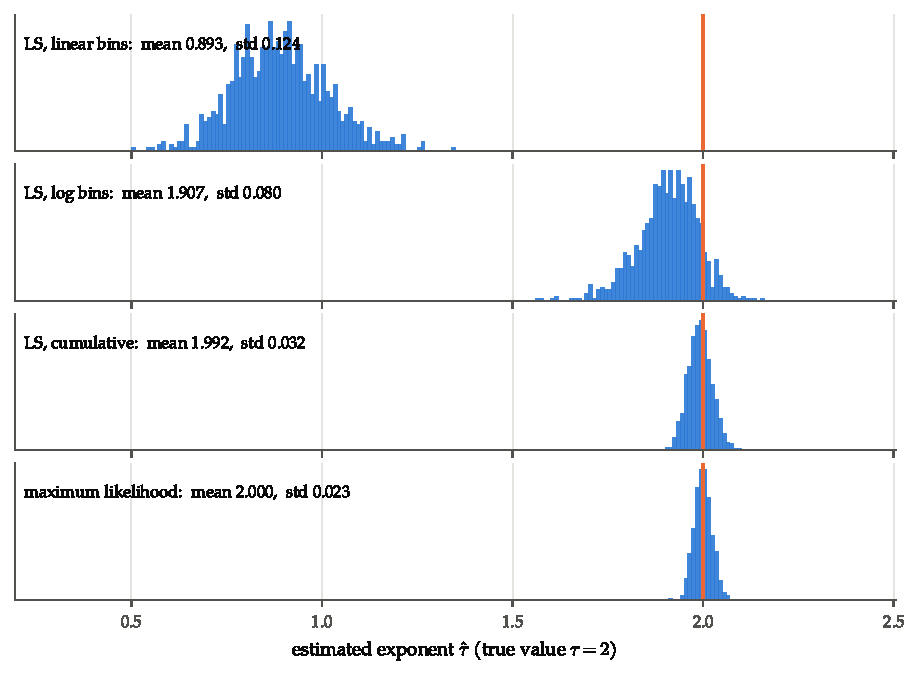
\includegraphics[width=\linewidth]{stats/estimators.pdf}
  \caption{Estimates of $\tau$ from 1000 independent synthetic samples of 2000 values with true exponent $\tau=2$
  (vertical line), using four methods.}
  \label{fig:estimators}
\end{figure}

Least squares on a linear histogram is useless: it does not even get close to the right answer. With logarithmic
bins the result is biased by about 5\%, and the spread is large. The cumulative distribution does better, but the
maximum-likelihood method, described next, is both unbiased and the most precise.

% ======================================================================
\section{Maximum likelihood}
\label{sec:mle}

\subsection{The idea}

Suppose we have a model for the distribution, $P(x\,|\,\tau)$, that depends on an unknown parameter $\tau$. For a
given value of $\tau$, the probability (density) of having observed exactly our data $x_1,\dots,x_N$ is, if the values are
independent,
\begin{equation}
  \mathcal L(\tau) = \prod_{i=1}^N P(x_i\,|\,\tau).
\end{equation}
Seen as a function of $\tau$, this is called the \emph{likelihood}. The \emph{maximum-likelihood estimate} $\hat\tau$ is the
value of $\tau$ that makes the observed data most probable. It is usually easier to maximise the logarithm,
$\ln\mathcal L = \sum_i \ln P(x_i\,|\,\tau)$, which has its maximum at the same place.

\subsection{Continuous power law}

For the normalised power law $P(x) = \frac{\tau-1}{x_{\min}}\left(\frac{x}{x_{\min}}\right)^{-\tau}$ on $x\ge x_{\min}$,
\begin{equation}
  \ln\mathcal L(\tau) = N\ln(\tau-1) - N\ln x_{\min} - \tau\sum_{i=1}^N \ln\frac{x_i}{x_{\min}} .
\end{equation}
Setting the derivative with respect to $\tau$ to zero,
\begin{equation}
  \frac{\dd\ln\mathcal L}{\dd\tau} = \frac{N}{\tau-1} - \sum_i\ln\frac{x_i}{x_{\min}} = 0
  \quad\Longrightarrow\quad
  \boxed{\;\hat\tau = 1 + \frac{N}{\sum_{i=1}^N \ln(x_i/x_{\min})}.\;}
  \label{eq:mle}
\end{equation}

\paragraph{Intuition.} Change variables to $u = \ln(x/x_{\min})$, the logarithm of the size. Since $\dd u = \dd x/x$,
\[
  P(u) = P(x)\frac{\dd x}{\dd u} = x\,P(x) = (\tau-1)\left(\frac{x}{x_{\min}}\right)^{1-\tau} = (\tau-1)\,e^{-(\tau-1)u}.
\]
The logarithm of a power-law variable is \emph{exponentially} distributed, with mean $1/(\tau-1)$. \Cref{eq:mle} simply
says: estimate $\tau-1$ as one over the average of $\ln(x/x_{\min})$. Every value contributes, each with the same weight;
nothing is binned and nothing is thrown away.

\paragraph{The error.} The width of the peak of $\ln\mathcal L$ tells how well $\tau$ is determined: a sharp peak means
that values of $\tau$ slightly different from $\hat\tau$ make the data much less probable. For large $N$, $\ln\mathcal L$
is close to a parabola near its maximum, and the standard error is
\begin{equation}
  \sigma_\tau = \left(-\frac{\dd^2\ln\mathcal L}{\dd\tau^2}\right)^{-1/2} = \left(\frac{N}{(\tau-1)^2}\right)^{-1/2}
  = \frac{\hat\tau-1}{\sqrt N} .
  \label{eq:mle-err}
\end{equation}
The error decreases as $1/\sqrt N$, as for any average. We checked that this error bar is correct by repeating the fit
on 400 independent synthetic samples: the true value lies within $\pm\sigma_\tau$ of the estimate in $68\%$ of the cases,
as it should for a Gaussian error.

\subsection{Discrete data}

Avalanche sizes are integers, and for small sizes the continuous formula is wrong: it treats all values between 1 and 2 as
if they were spread over the interval, whereas the data sit exactly at 1. For integers the normalised power law is
\begin{equation}
  P(s) = \frac{s^{-\tau}}{\zeta(\tau, s_{\min})}, \qquad
  \zeta(\tau, s_{\min}) = \sum_{s=s_{\min}}^{\infty} s^{-\tau},
\end{equation}
where $\zeta(\tau, s_{\min})$ is the \emph{Hurwitz zeta function}, available in standard numerical libraries. The
log-likelihood
\begin{equation}
  \ln\mathcal L(\tau) = -N\ln\zeta(\tau,s_{\min}) - \tau\sum_i\ln s_i
\end{equation}
has no closed-form maximum, but it is easily maximised numerically, and the error again follows from its curvature. The
difference is not small: for $10^5$ integers drawn from $P(s)\propto s^{-1.7}$, $s\ge1$, the continuous formula gives
$\hat\tau=2.04$, while the discrete likelihood gives the correct $1.701\pm0.002$.

\subsection{Fitting a window: the truncated power law}

Real distributions follow a power law only up to a cutoff. If a fit assumes that the power law continues to infinity, the
missing tail is interpreted as a steeper decay, and $\hat\tau$ comes out too large. For $10^5$ values drawn from a power law
with $\tau=1.25$ that ends sharply at $x=1000$, the untruncated fit gives $\hat\tau = 1.40$. The correct procedure is to fit
only a window $[x_{\min}, x_{\max}]$ and to normalise the model on that window:
\begin{equation}
  P(x) = \frac{x^{-\tau}}{Z(\tau)}, \qquad Z(\tau) = \int_{x_{\min}}^{x_{\max}} x^{-\tau}\,\dd x =
  \frac{x_{\min}^{1-\tau} - x_{\max}^{1-\tau}}{\tau-1}
\end{equation}
(for integers, $Z = \zeta(\tau, s_{\min}) - \zeta(\tau, s_{\max}+1)$). With this model the same data give $1.249\pm0.002$.
A useful by-product is that in a window the exponent can take any value, also $\tau\le1$, which is impossible for an
untruncated power law.

% ======================================================================
\section{Where does the power law start? Goodness of fit}
\label{sec:xmin}

\subsection{Choosing the lower limit}

At small sizes, lattice effects make the distribution deviate from the power law. The lower limit $x_{\min}$ of the fit must
be chosen above this region. Choosing it by eye is subjective; a systematic method is to choose the $x_{\min}$ for which the
fitted power law is closest to the data~\cite{Clauset2009}. ``Closest'' is measured by the \emph{Kolmogorov--Smirnov (KS)
distance}
\begin{equation}
  D_{\mathrm{KS}} = \max_{x\ge x_{\min}}\left|\hat F(x) - F_{\text{model}}(x)\right| ,
\end{equation}
the largest vertical gap between the measured cumulative distribution of the data above $x_{\min}$ and that of the fitted
power law. For each candidate $x_{\min}$ we fit $\tau$ by maximum likelihood and compute $D_{\mathrm{KS}}$; the best $x_{\min}$ is
the one with the smallest distance.

\Cref{fig:xmin} shows how this works on synthetic data: an exponential ``body'' below $x=10$ followed by a power-law tail with
$\tau=2.5$. If the fit starts at $x_{\min}=1$, the body is mistaken for part of the power law and $\hat\tau = \stxminTauOne$.
The KS distance drops sharply at the true onset; its minimum is at $x_{\min}=\stxminBest$, where
$\hat\tau=\stxminTau\pm\stxminErr$. Above the onset, $\hat\tau$ is flat in $x_{\min}$ (right panel); a flat region of this kind is
itself a good sign that a power law is present.

\begin{figure}[t]
  \centering
  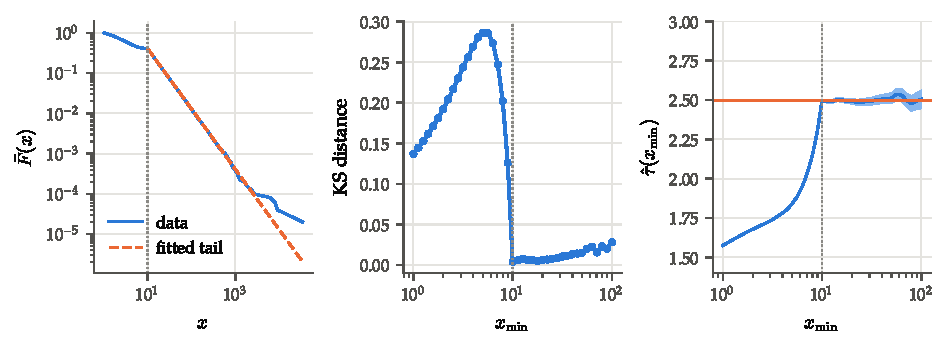
\includegraphics[width=\linewidth]{stats/xmin.pdf}
  \caption{Choosing $x_{\min}$. Synthetic data with an exponential body below 10 and a power-law tail with $\tau=2.5$. Left:
  cumulative distribution and the fitted tail. Middle: KS distance as a function of the lower limit. Right: fitted exponent with
  its error band; the horizontal line is the true value.}
  \label{fig:xmin}
\end{figure}

\subsection{Is it a power law at all?}

A fit always returns a number, even if the data do not follow a power law. To test the hypothesis itself we ask: if the data
really came from the fitted power law, how often would a sample of the same size have a KS distance as large as the one observed?
This probability, the $p$-value, is computed by a \emph{parametric bootstrap}~\cite{Efron1979,Clauset2009}:
\begin{enumerate}[nosep]
  \item fit the data, obtaining $\hat\tau$ and the observed distance $D_{\mathrm{obs}}$;
  \item draw many synthetic samples, of the same size, from the power law with exponent $\hat\tau$;
  \item fit each synthetic sample in the same way and compute its KS distance;
  \item the $p$-value is the fraction of synthetic samples whose distance is at least $D_{\mathrm{obs}}$.
\end{enumerate}
If $p$ is small (we use $p<0.1$), data of this kind rarely come from a power law, and the hypothesis is rejected. A large $p$
does not prove that the distribution is a power law; it only says that the data are consistent with one.

% ======================================================================
\section{Statistical errors of correlated data}
\label{sec:correlated}

\subsection{Why independence fails}

The error formula $\sigma/\sqrt N$ for a mean assumes independent values. In a simulation of a sandpile or of a fault, events are
produced one after the other by the same system, and the state left behind by one event is the starting state of the next. Events
can therefore be correlated in time. The \emph{autocorrelation function}
\begin{equation}
  C(\Delta) = \frac{\avg{(x_t-\avg{x})(x_{t+\Delta}-\avg{x})}}{\avg{(x-\avg{x})^2}}
\end{equation}
measures how similar two events separated by $\Delta$ steps are; $C(0)=1$, and $C(\Delta)=0$ for independent events. For a series
of $N$ correlated values the variance of the mean is
\begin{equation}
  \mathrm{Var}(\bar x) = \frac{\sigma^2}{N}\Bigl(1 + 2\sum_{\Delta\ge1} C(\Delta)\Bigr),
  \label{eq:var-corr}
\end{equation}
so positive correlations increase the error and negative ones decrease it. Even very small correlations matter if they last
long, because \cref{eq:var-corr} sums them over all lags.

\subsection{The blocking method}

A practical way to obtain the correct error without computing $C(\Delta)$ is the \emph{blocking} method~\cite{FlyvbjergPetersen1989}.
Divide the series into consecutive blocks of length $b$, compute the mean of each block, and estimate the error of the overall
mean from the scatter of the block means as if they were independent. For $b=1$ this is the naive error. As $b$ grows beyond the
time over which events are correlated, the block means become independent, and the estimate stops changing: the value on this
\emph{plateau} is the correct error. For quantities other than the mean, such as exponents, the same idea leads to the \emph{block
bootstrap}: resample whole blocks (with replacement) many times, recompute the quantity each time, and use the spread of the
results as the error.

\subsection{An example: the BTW sandpile}

\Cref{fig:correlations} shows the autocorrelation of avalanche sizes in the two-dimensional BTW model with $L=64$. It is tiny,
$C(1)=\stcorrAcfOne$, but negative and long-lived. The blocking analysis (right) shows that the correct error of $\avg{s}$ is not
the naive one but only about $\stcorrSeed$ of it, a factor of seven smaller.

\begin{figure}[t]
  \centering
  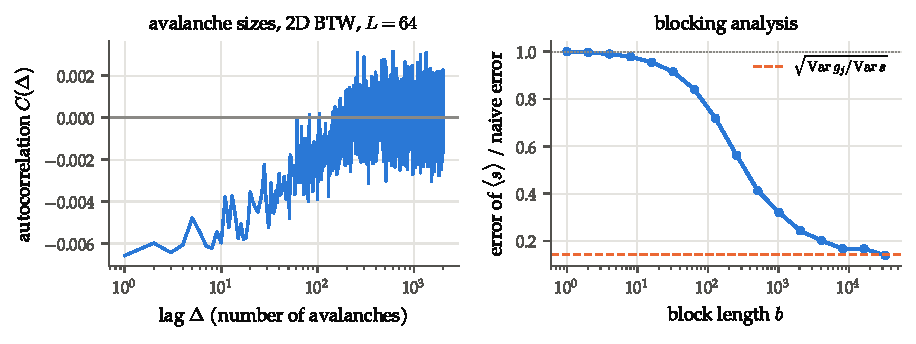
\includegraphics[width=\linewidth]{stats/correlations.pdf}
  \caption{Two-dimensional BTW model, $L=64$, $10^6$ avalanches. Left: autocorrelation of the sizes of consecutive avalanches.
  Right: error of the mean size from the blocking method, in units of the naive error $\sigma/\sqrt N$; the dashed line is the
  prediction of \cref{eq:block-sum}.}
  \label{fig:correlations}
\end{figure}

This surprising result has an exact explanation, which shows the power of the balance equation \cref{eq:balance}. Add up the balance
equations of $b$ consecutive grains, added at sites $j_1,\dots,j_b$. The heights at the end of the block are
\[
  z^{\text{end}} = z^{\text{start}} + \sum_{t=1}^b e_{j_t} - \Delta\,N_{\text{block}},
\]
where $N_{\text{block}}$ is the vector of the total numbers of topplings at each site during the block. Solving for $N_{\text{block}}$ with
$G=\Delta^{-1}$ and summing over sites,
\begin{equation}
  \sum_{t=1}^b s_t = \sum_{t=1}^b g_{j_t} + \sum_{i,m} G_{im}\bigl(z_m^{\text{start}} - z_m^{\text{end}}\bigr).
  \label{eq:block-sum}
\end{equation}
The second term is bounded, since all heights lie between 0 and 3; divided by $b$, it disappears for long blocks. The first term is a
sum of $b$ independent random numbers, because the sites $j_t$ are chosen independently. So for long blocks the fluctuation of the mean
size comes only from the randomness of \emph{where} grains are dropped, not from the avalanches themselves, and the error of the mean is
$\sqrt{\mathrm{Var}(g_j)/b}$ instead of $\sqrt{\mathrm{Var}(s)/b}$. For $L=64$ the ratio $\sqrt{\mathrm{Var}(g_j)/\mathrm{Var}(s)}$ is
$\stcorrSeed$, exactly the plateau of \cref{fig:correlations}. The anticorrelation has a simple physical meaning: an unusually large
avalanche removes many grains, and the following avalanches are smaller until the pile has been refilled.

This exact cancellation is special to a conservative sandpile, but the lesson is general: errors must always be estimated with a method
that accounts for correlations, such as blocking or the block bootstrap. Depending on the sign of the correlations, the naive error can be
too large or too small.

% ======================================================================
\section{Finite-size scaling}
\label{sec:fss}

\subsection{The scaling hypothesis}

In a finite system the power law is cut off at a size that grows with the system. The \emph{finite-size scaling} hypothesis states that
the system size $L$ is the \emph{only} scale in the problem besides the microscopic one, so that the distribution has the form
\begin{equation}
  P(s;L) = s^{-\tau}\,\mathcal G\!\left(\frac{s}{L^{D}}\right)
  \label{eq:fss3}
\end{equation}
for $s$ well above the lattice scale, with a cutoff function $\mathcal G$ that does not depend on $L$. This is the same form as the
percolation cluster distribution \cref{eq:perc-scaling}, with $L$ in place of the correlation length $\xi$: in a finite critical system,
the system size plays the role of the correlation length. In the Burridge--Knopoff model the roles will be reversed: the system can be made
much longer than the correlation length, and $\xi$ (set by the model parameters) will take the place of $L$.

\Cref{eq:fss3} has three consequences that can be tested with data from several system sizes.

\subsection{Data collapse}

Multiply \cref{eq:fss3} by $s^\tau$:
\begin{equation}
  s^{\tau}P(s;L) = \mathcal G\!\left(\frac{s}{L^{D}}\right).
\end{equation}
The right-hand side depends on $s$ and $L$ only through the combination $s/L^D$. So if we plot $s^\tau P(s;L)$ against $s/L^{D}$ for
several $L$, with the correct $\tau$ and $D$, all curves fall on top of each other: the data \emph{collapse} onto the single curve
$\mathcal G$. With wrong exponents, the curves are shifted or tilted relative to each other.

To make this quantitative, we compare the rescaled curves on a common grid of $s/L^{D}$ and compute how far they are from their (error-weighted)
mean, in units of their statistical errors~\cite{BhattacharjeeSeno2001}:
\begin{equation}
  \chi^2 = \frac{1}{N_{\text{grid}}}\sum_{\text{grid points}}\;\frac{1}{N_L-1}\sum_{L}\frac{\bigl(y_L - \bar y\bigr)^2}{\sigma_L^2},
\end{equation}
where $y_L = \ln[s^{\tau}P(s;L)]$ interpolated at the grid point, $\sigma_L$ its statistical error, $\bar y$ the weighted mean over the $N_L$
system sizes. If the curves agree within their statistical noise, $\chi^2\approx1$. The best exponents are those that minimise $\chi^2$. For
synthetic data with $\tau=1.6$ and $D=2$ (an exponential cutoff at $s = L^2$, $L$ from 32 to 256), this procedure gives
$\tau = \stsynTau$, $D=\stsynD$ with $\chi^2=\stsynCost$: a perfect collapse (\cref{fig:collapse}, left).

\subsection{Moments}

As derived in \cref{sec:btw2d}, \cref{eq:fss3} implies $\avg{s^q}\propto L^{\sigma(q)}$ with $\sigma(q) = D(q+1-\tau)$ for $q>\tau-1$. The
moment exponents are obtained as slopes of $\ln\avg{s^q}$ against $\ln L$, and their errors with the block bootstrap of
\cref{sec:correlated}. The slope of $\sigma(q)$ gives $D$, and its intercept gives $\tau$.

\subsection{Effective exponents}

Instead of fitting one exponent to all the data, it is often more informative to fit the truncated power law in a sliding window, for
example one decade $[s, 10s]$, and plot the resulting \emph{effective exponent} $\tau_{\text{eff}}$ against the position of the window.
For a true power law $\tau_{\text{eff}}$ is constant; deviations show where, and how strongly, the distribution bends.

\subsection{Corrections to scaling}

\Cref{eq:fss3} is an \emph{asymptotic} statement, valid for $L\to\infty$ and $s\to\infty$. At finite sizes there are corrections, and
when $\tau$ is close to 1 they can be surprisingly large. The reason is the normalisation. For \cref{eq:fss3} to be a normalised distribution
starting at $s=1$,
\[
  \int_1^\infty s^{-\tau}\mathcal G(s/s_c)\,\dd s \approx \frac{1}{\tau-1} - c\, s_c^{-(\tau-1)}
\]
must equal 1 for every $L$ (here $s_c = L^D$ and $c$ is a positive constant). The second term is a correction that decays as
$s_c^{-(\tau-1)}$. For $\tau=1.3$ this is $s_c^{-0.3}$: making the cutoff ten times larger reduces the correction only by a factor
$10^{0.3}\approx2$. To keep the distribution normalised, its overall amplitude must therefore change slowly with $L$, and all exponents
measured from a range of $L$ are affected.

\Cref{fig:corrections} shows this for a case where everything is known exactly: the moments of $P(s)\propto s^{-1.3}e^{-s/L^2}$, computed by
numerical integration. The local slopes $\dd\ln\avg{s^q}/\dd\ln L$ approach their asymptotic values $\sigma(q)=D(q+1-\tau)$ only slowly from
below; for $L$ around 30 the slope for $q=1$ is still about $10\%$ too small. A common way to handle this is to allow a correction term,
$\avg{s^q} = a\,L^{\sigma(q)}(1 + b\,L^{-\omega})$, or to compute effective exponents from pairs of neighbouring sizes and watch how they
change as $L$ grows.

\begin{figure}[t]
  \centering
  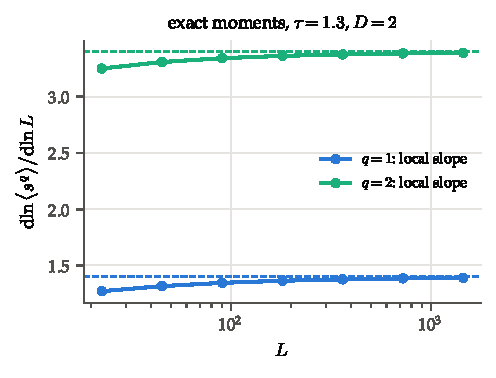
\includegraphics[width=0.55\linewidth]{stats/corrections.pdf}
  \caption{Corrections to scaling in a case known exactly: local slopes of the moments of $P(s)\propto s^{-1.3}e^{-s/L^2}$ between
  neighbouring system sizes (points), and their asymptotic values $D(q+1-\tau)$ (dashed lines).}
  \label{fig:corrections}
\end{figure}

% ======================================================================
\section{Application: the two-dimensional BTW sandpile}
\label{sec:btw2d-exponents}

We now apply these tools to the BTW data of \cref{sec:btw2d} ($L=32$ to 512, $10^6$ avalanches each). The results are a lesson in caution.

\paragraph{Effective exponents.} \Cref{fig:effective} (left) shows $\tau_{\text{eff}}$ from truncated fits in one-decade windows. For every $L$
there is a range in which $\tau_{\text{eff}}$ rises only slowly, from about $1.0$ to $1.13$, followed by a sharp rise at the cutoff. For
$L=512$, a fit of the window $[10^2,10^4]$ gives $\tau=\stbtwWinTau\pm\stbtwWinErr$ with a goodness-of-fit $p$-value of $\stbtwWinP$: in this
window the data are statistically consistent with a pure power law. The right panel shows what happens if the cutoff is ignored and all
$s\ge s_{\min}$ are fitted: $\hat\tau$ is always too large and keeps increasing with $s_{\min}$, so no stable value can be read off.

\begin{figure}[t]
  \centering
  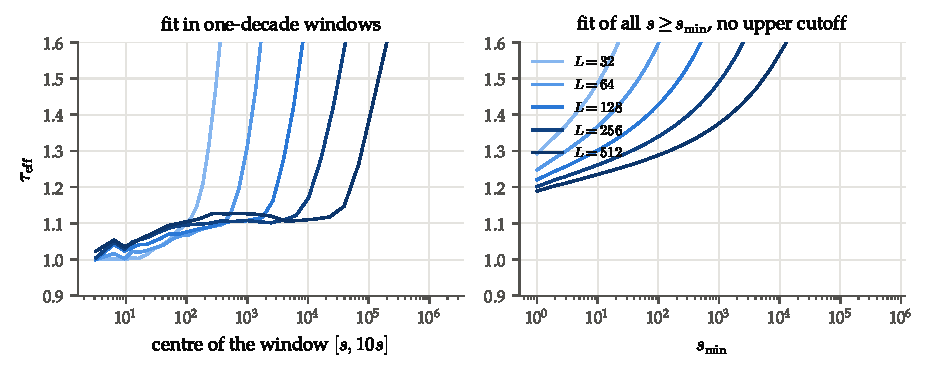
\includegraphics[width=\linewidth]{stats/effective_exponent.pdf}
  \caption{Effective exponents of the avalanche-size distribution of the two-dimensional BTW model. Left: truncated maximum-likelihood fits in
  windows $[s,10s]$, plotted at the centre of the window. Right: untruncated fits of all $s\ge s_{\min}$.}
  \label{fig:effective}
\end{figure}

\paragraph{Moments and collapse.} The moment analysis of \cref{sec:btw2d} gave $D=\stmomD$ and, through $D(2-\tau)=2$, $\tau=\stmomTau$, much
larger than the window value $1.12$. With these exponents the curves do not collapse (\cref{fig:collapse}, middle): their slopes at small $s/L^D$
differ visibly, and $\chi^2\approx\stmomCost$. Minimising $\chi^2$ over $\tau$ and $D$ does not rescue the collapse, and the result depends on which part
of the curves is used. Using the whole range gives $\tau=\stcollATau$, $D=\stcollAD$ ($\chi^2=\stcollACost$); using only the region near the cutoff
($s/L^D>10^{-2}$) gives $\tau=\stcollBTau$, $D=\stcollBD$ ($\chi^2=\stcollBCost$). Finally, the effective $D$ computed from pairs of neighbouring
sizes (\cref{fig:collapse}, right) is $\stDloc$ for the four pairs, with bootstrap errors $\stDerr$. These values scatter around the literature value
$2.73$~\cite{LubeckUsadel1997} but show no clear convergence.

\begin{figure}[t]
  \centering
  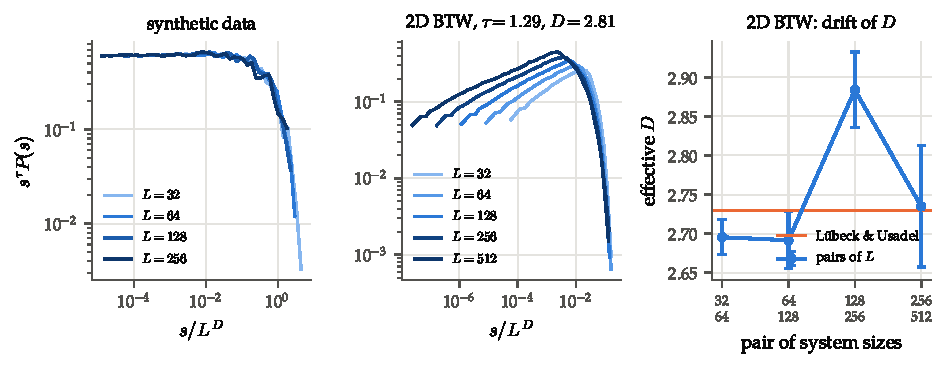
\includegraphics[width=\linewidth]{stats/collapse.pdf}
  \caption{Data collapse. Left: synthetic data that obey \cref{eq:fss3} exactly, collapsed with the fitted exponents. Middle: the two-dimensional
  BTW model, rescaled with the exponents from the moment analysis; the curves do not collapse. Right: effective fractal dimension $D$ of the BTW
  model obtained from pairs of neighbouring system sizes, with block-bootstrap errors, and the literature value.}
  \label{fig:collapse}
\end{figure}

\paragraph{Interpretation.} All the methods work correctly on synthetic data that obey \cref{eq:fss3}. Their disagreement on the BTW model is
therefore a property of the model, not of the methods: the BTW sandpile does not follow simple finite-size scaling. Small avalanches (single waves of
topplings) and large avalanches (many waves stacked on top of each other) scale differently, which is the multifractality mentioned in
\cref{sec:btw2d}~\cite{Tebaldi1999}. A single number $\tau$ cannot describe all scales, and different methods weight different scales. The general
lesson for this thesis is that an exponent should never be reported from one method alone: a value is trustworthy only when independent methods
(window fits, moments, collapse) agree within their errors.

% ======================================================================
\section{The procedure used in this thesis}
\label{sec:protocol}

For every model studied in the following chapters, distributions and exponents are obtained as follows.
\begin{enumerate}
  \item \textbf{Stationarity.} Start from a well-defined initial state, discard a transient long enough for averages to stop drifting, and record
    the events in time order.
  \item \textbf{Display.} Show densities with logarithmic bins (integer-aware for integer data) and Poisson error bars, and cumulative distributions
    for the tails. Magnitude histograms in $\mu=\ln M$ are translated with $\tau = 1+b$.
  \item \textbf{Exponents.} Estimate $\tau$ by maximum likelihood of a (discrete, if appropriate) truncated power law in a window. Choose the lower
    limit by the KS distance, test the fit with a bootstrap $p$-value, and show the effective exponent in sliding windows to make the range of validity
    visible.
  \item \textbf{Scaling.} Use several values of the parameter that sets the cutoff (the system size $L$ for sandpiles, the correlation length for the
    Burridge--Knopoff model). Measure moment exponents and test data collapse with the $\chi^2$ measure, and compute effective exponents from neighbouring
    values of the parameter to judge corrections to scaling.
  \item \textbf{Errors.} Estimate statistical errors with the block bootstrap. Report the spread between different methods as a systematic uncertainty.
  \item \textbf{Validation.} Before applying any analysis to new data, check that it returns the known answer on synthetic data generated with similar
    exponents, ranges and sample sizes.
\end{enumerate}
